\documentclass[a4paper, 14pt]{article}
\usepackage[T2A]{fontenc}
\usepackage[utf8]{inputenc}
\usepackage[english,russian]{babel}
\usepackage[top = 2cm, bottom = 2 cm]{geometry}
\usepackage{cmap}
\usepackage{graphicx}
\usepackage{listings}
\usepackage{color}
\usepackage{amsmath}
\usepackage{pgfplots}
\usepackage{url}
\usepackage{tikz}
\usepackage{float}
\usepackage{multirow}

\usepackage{titlesec}
\titleformat*{\section}{\LARGE\bfseries}
\titleformat*{\subsection}{\Large\bfseries}
\titleformat*{\subsubsection}{\large\bfseries}
\titleformat*{\paragraph}{\large\bfseries}
\titleformat*{\subparagraph}{\large\bfseries}

\lstset{
	language=Python, 
	numbers=left,   
	frame=single, 
	escapebegin=\begin{russian}\commentfont,
    escapeend=\end{russian},
    breaklines=true,   
    breakatwhitespace=true,
	literate={а}{{\selectfont\char224}}1
	{б}{{\selectfont\char225}}1
	{в}{{\selectfont\char226}}1
	{г}{{\selectfont\char227}}1
	{д}{{\selectfont\char228}}1
	{е}{{\selectfont\char229}}1
	{ё}{{\"e}}1
	{ж}{{\selectfont\char230}}1
	{з}{{\selectfont\char231}}1
	{и}{{\selectfont\char232}}1
	{й}{{\selectfont\char233}}1
	{к}{{\selectfont\char234}}1
	{л}{{\selectfont\char235}}1
	{м}{{\selectfont\char236}}1
	{н}{{\selectfont\char237}}1
	{о}{{\selectfont\char238}}1
	{п}{{\selectfont\char239}}1
	{р}{{\selectfont\char240}}1
	{с}{{\selectfont\char241}}1
	{т}{{\selectfont\char242}}1
	{у}{{\selectfont\char243}}1
	{ф}{{\selectfont\char244}}1
	{х}{{\selectfont\char245}}1
	{ц}{{\selectfont\char246}}1
	{ч}{{\selectfont\char247}}1
	{ш}{{\selectfont\char248}}1
	{щ}{{\selectfont\char249}}1
	{ъ}{{\selectfont\char250}}1
	{ы}{{\selectfont\char251}}1
	{ь}{{\selectfont\char252}}1
	{э}{{\selectfont\char253}}1
	{ю}{{\selectfont\char254}}1
	{я}{{\selectfont\char255}}1
	{А}{{\selectfont\char192}}1
	{Б}{{\selectfont\char193}}1
	{В}{{\selectfont\char194}}1
	{Г}{{\selectfont\char195}}1
	{Д}{{\selectfont\char196}}1
	{Е}{{\selectfont\char197}}1
	{Ё}{{\"E}}1
	{Ж}{{\selectfont\char198}}1
	{З}{{\selectfont\char199}}1
	{И}{{\selectfont\char200}}1
	{Й}{{\selectfont\char201}}1
	{К}{{\selectfont\char202}}1
	{Л}{{\selectfont\char203}}1
	{М}{{\selectfont\char204}}1
	{Н}{{\selectfont\char205}}1
	{О}{{\selectfont\char206}}1
	{П}{{\selectfont\char207}}1
	{Р}{{\selectfont\char208}}1
	{С}{{\selectfont\char209}}1
	{Т}{{\selectfont\char210}}1
	{У}{{\selectfont\char211}}1
	{Ф}{{\selectfont\char212}}1
	{Х}{{\selectfont\char213}}1
	{Ц}{{\selectfont\char214}}1
	{Ч}{{\selectfont\char215}}1
	{Ш}{{\selectfont\char216}}1
	{Щ}{{\selectfont\char217}}1
	{Ъ}{{\selectfont\char218}}1
	{Ы}{{\selectfont\char219}}1
	{Ь}{{\selectfont\char220}}1
	{Э}{{\selectfont\char221}}1
	{Ю}{{\selectfont\char222}}1
	{Я}{{\selectfont\char223}}1
}

\newcommand{\biglisting}[1]{%
	\lstinputlisting[numbers=left]{#1}%
}

\begin{document}

	\textbf{Цель работы:} получение навыков разработки  алгоритмов решения смешанной краевой задачи при реализации моделей, построенных на квазилинейном уравнении параболического типа. \\
	
	
	\section*{Теоретическая часть}
	
	Задана математическая модель.\\
	Уравнение для функции $T(x, t)$
	\begin{equation}
c(T)\frac{\partial T}{\partial t}=\frac{\partial}{\partial x}\bigg(k(T)\frac{\partial T}{\partial x}\bigg)-\frac{2}{R}\alpha(x)T+\frac{2T_0}{R}\alpha(x)
\end{equation}

Краевые условия
$$
 \begin{cases}
 t=0, ~T(x,0)=T_0
   \\
   x=0, ~-k(T(0))\frac{\partial T}{\partial x}=F_0
   \\
   x =l,~-k(l)\frac{\partial T}{\partial x}=\alpha_N(T(l)-T_0)
 \end{cases}
$$

В обозначениях уравнения (14.1) лекции №14
$$p(x)=\frac{2}{R}\alpha(x)$$
$$f(x)=\frac{2T_0}{R}\alpha(x)$$

Функция $\alpha(x)$ задана уравнением:

$$\alpha(x)=\frac{c}{x-d}$$

Константы $c$ и $d$  из условий $\alpha(0) = a_0, \alpha(l) = a_N, $

$$c=-\alpha_0d=\frac{\alpha_0\alpha_Nl}{\alpha_0-\alpha_N}$$
$$d = \frac{\alpha_Nl}{\alpha_N-\alpha_0}$$

Разностная схема

\begin{equation}
\begin{aligned}
&\buildrel\,\,\frown\over{A}_n\buildrel\,\,\frown\over{y}_{n-1}-\buildrel\,\,\frown\over{B}_n\buildrel\,\,\frown\over{y}_n+\buildrel\,\,\frown\over{D}_n\buildrel\,\,\frown\over{y}_{n+1}=-\buildrel\,\,\frown\over{F}_n, 1\le n\le N-1\\
&\buildrel\,\,\frown\over{A}_n=\buildrel\,\,\frown\over{\chi}_{n-\frac{1}{2}}\frac{\tau}{h},\\
&\buildrel\,\,\frown\over{B}_n=\buildrel\,\,\frown\over{A}_n+\buildrel\,\,\frown\over{D}_n+\buildrel\,\,\frown\over{c}_nh+p_nh\tau,\\
& \buildrel\,\,\frown\over{D}_n=\buildrel\,\,\frown\over{\chi}_{n+\frac{1}{2}}\frac{\tau}{h}, \\
&\buildrel\,\,\frown\over{F}_n=f_nh\tau+\buildrel\,\,\frown\over{c}_ny_nh\\
\end{aligned}
\end{equation}\\

Разностные аналоги краевых условий при $x = 0$ (получены в Лекции №14)

\begin{multline}
\bigg(\frac{h}{8}\buildrel\,\,\frown\over{c}_{\frac{1}{2}}+ \frac{h}{4}\buildrel\,\,\frown\over{c}_0+\buildrel\,\,\frown\over{\chi}_{\frac{1}{2}}\frac{\tau}{h}+\frac{\tau h}{8}p_{\frac{1}{2}}+\frac{\tau h}{4}p_0\bigg)\buildrel\,\,\frown\over{y}_0+\bigg(\frac{h}{8}\buildrel\,\,\frown\over{c}_{\frac{1}{2}}-\buildrel\,\,\frown\over{\chi}_{\frac{1}{2}}\frac{\tau}{h}+\frac{\tau h}{8}p_{\frac{1}{2}}\bigg)\buildrel\,\,\frown\over{y}_1=\\
= \frac{h}{8}\buildrel\,\,\frown\over{c}_{\frac{1}{2}}(y_0+y_1)+\frac{h}{4}\buildrel\,\,\frown\over{c}_0y_0+\buildrel\,\,\frown\over{F}\tau+\frac{\tau h}{4}(\buildrel\,\,\frown\over{f}_{\frac{1}{2}}+\buildrel\,\,\frown\over{c}_0)
\end{multline}

Получим интегро-интерполяционным методом разностный аналог краевого условия при  $x = l$. Для этого обозначим $F=-k(T)\frac{\partial T}{\partial x}$ и учтем то, что поток
$$
\buildrel\,\,\frown\over{F}_N=\alpha_N(\buildrel\,\,\frown\over{y}_N-T_0),
\buildrel\,\,\frown\over{F}_{N-\frac{1}{2}}=\buildrel\,\,\frown\over{\chi}_{N-\frac{1}{2}}\frac{\buildrel\,\,\frown\over{y}_{N-1}-\buildrel\,\,\frown\over{y}_N}{h}
$$

Проинтегрируем уравнение (1) на отрезке $[x_{N-\frac{1}{2}},x_N]$

\begin{multline*}
\int^{x_N}_{x_{N-{\frac{1}{2}}}}dx=-\int^{t_{m+1}}_{t_{m}}dt\int^{x_N}_{x_{N-{\frac{1}{2}}}}\frac{\partial F}{\partial x}dx-\int^{x_N}_{x_{N-{\frac{1}{2}}}}dx\int^{t_{m+1}}_{t_{m}}p(x)Tdt+\\
+\int^{x_N}_{x_{N-{\frac{1}{2}}}}dx\int^{t_{m+1}}_{t_{m}}f(T)dt
\end{multline*}

\begin{multline*}
\int^{x_N}_{x_{N-{\frac{1}{2}}}}\buildrel\,\,\frown\over{c}(\buildrel\,\,\frown\over{T}-T)dx = 
-\int^{t_{m+1}}_{t_{m}}(F_N-F_{N-\frac{1}{2}})dt-\int^{x_N}_{x_{N-{\frac{1}{2}}}}p\buildrel\,\,\frown\over{T}\tau dx+\int^{x_N}_{x_{N-{\frac{1}{2}}}}\buildrel\,\,\frown\over{f}\tau dx
\end{multline*}

\begin{multline*}
\big(\buildrel\,\,\frown\over{c}_{N}(\buildrel\,\,\frown\over{y}_N-y_N) + 
\buildrel\,\,\frown\over{c}_{N-\frac{1}{2}}(\buildrel\,\,\frown\over{y}_{N-\frac{1}{2}} -
y_{N-\frac{1}{2}})\big)\frac{h}{4} = 
-\tau(\buildrel\,\,\frown\over{F}_N - 
\buildrel\,\,\frown\over{F}_{N-\frac{1}{2}})-\\
-\big(p_N\buildrel\,\,\frown\over{y}_N +
p_{N-\frac{1}{2}}\buildrel\,\,\frown\over{y}_{N -
\frac{1}{2}}\big)\tau\frac{h}{4} +
(\buildrel\,\,\frown\over{f}_N +
\buildrel\,\,\frown\over{f}_{N-\frac{1}{2}})\tau \frac{h}{4}
\end{multline*}

\begin{multline*}
\frac{h}{4}\buildrel\,\,\frown\over{c}_{N}\buildrel\,\,\frown\over{y}_N - 
\frac{h}{4}\buildrel\,\,\frown\over{c}_{N}y_N+
 \frac{h}{8}\buildrel\,\,\frown\over{c}_{N-\frac{1}{2}}\buildrel\,\,\frown\over{y}_{N} + 
\frac{h}{8}\buildrel\,\,\frown\over{c}_{N-\frac{1}{2}\buildrel\,\,\frown\over{y}_{N-1}} - 
\frac{h}{8}\buildrel\,\,\frown\over{c}_{N-\frac{1}{2}}{y}_{N}\-\\
-\frac{h}{8}\buildrel\,\,\frown\over{c}_{N-\frac{1}{2}}{y}_{N-1} = 
-\tau\alpha_N\buildrel\,\,\frown\over{y}_N+\tau\alpha_NT_0 +
\tau\buildrel\,\,\frown\over{\chi}_{N-\frac{1}{2}}\frac{\buildrel\,\,\frown\over{y}_{N-1}}{h} - 
\tau\buildrel\,\,\frown\over{\chi}_{N-\frac{1}{2}}\frac{\buildrel\,\,\frown\over{y}_{N}}{h}-\\
-p_N\buildrel\,\,\frown\over{y}_N\tau\frac{h}{4} - 
p_{N-\frac{1}{2}}\buildrel\,\,\frown\over{y}_{N}\tau\frac{h}{8} - 
p_{N-\frac{1}{2}}\buildrel\,\,\frown\over{y}_{N-1}\tau\frac{h}{8} +
(\buildrel\,\,\frown\over{f}_N+\buildrel\,\,\frown\over{f}_{N-\frac{1}{2}})\tau \frac{h}{4}
\end{multline*}

\begin{multline}
\buildrel\,\,\frown\over{y}_{N-1}\bigg(\buildrel\,\,\frown\over{c}_{N-\frac{1}{2}}\frac{h}{8}  - 
\frac{\tau\buildrel\,\,\frown\over{\chi}_{N-\frac{1}{2}}}{h} + 
p_{N-\frac{1}{2}}\tau\frac{h}{8}  \bigg)+\\
+ \buildrel\,\,\frown\over{y}_N\bigg( \buildrel\,\,\frown\over{c}_{N}\frac{h}{4} + 
\buildrel\,\,\frown\over{c}_{N-\frac{1}{2}}\frac{h}{8} + 
\tau\alpha_N +
\frac{ \tau\buildrel\,\,\frown\over{\chi}_{N-\frac{1}{2}}}{h} +
p_N\tau\frac{h}{4}+p_{N-\frac{1}{2}}\tau\frac{h}{8} \bigg)=\\
=\buildrel\,\,\frown\over{c}_{N-\frac{1}{2}}\bigg({y}_{N}\frac{h}{8} +
{y}_{N-1}\frac{h}{8} \bigg) +
\buildrel\,\,\frown\over{c}_{N}y_N\frac{h}{4} +
\tau\alpha_NT_0 +
(\buildrel\,\,\frown\over{f}_N +
\buildrel\,\,\frown\over{f}_{N-\frac{1}{2}})\tau \frac{h}{4}
\end{multline}

Из полученных краевых условий находим коэффициенты $K_0,~K_N,~M_0,~M_N,~P_0,~P_N$. 


\begin{equation}
\begin{cases}
\buildrel\,\,\frown\over{K}_0\buildrel\,\,\frown\over{y}_0+\buildrel\,\,\frown\over{M}_0\buildrel\,\,\frown\over{y}_1=\buildrel\,\,\frown\over{P}_0\\
\buildrel\,\,\frown\over{A}_n\buildrel\,\,\frown\over{y}_{n-1}-\buildrel\,\,\frown\over{B}_n\buildrel\,\,\frown\over{y}_n+\buildrel\,\,\frown\over{D}_n\buildrel\,\,\frown\over{y}_{n+1}=-\buildrel\,\,\frown\over{F}_n, 1\le n\le N-1\\
\buildrel\,\,\frown\over{K}_N\buildrel\,\,\frown\over{y}_N+\buildrel\,\,\frown\over{M}_{N-1}\buildrel\,\,\frown\over{y}_{N-1}=\buildrel\,\,\frown\over{P}_N\\
\end{cases}
\end{equation}

Данная система решается методом итераций. Обозначим текущую итерацию $s$, а предыдущую $s - 1$ 

$${A}_n^{s-1}{y}_{n+1}^{s}-{B}_n^{s-1}{y}_n^{s}+{D}^{s-1}_n{y}_{n-1}^{s}=-{F}^{s-1}_n$$\\

Значения параметров\\

$k(T) = a_1(b_1 + c_1 T^{m_1}), \frac{\text{Вт}}{\text{см К}},$\\
 $c(T) = a_2 + b_2 T^{m_2} - \frac{c_2}{T^2}, \frac{\text{Дж}}{\text{см}^3 \text{К}},$ \\
$a_1 = 0.0134,$\\
$b_1 = 1,$\\
$ c_1 = 4.35 \cdot 10^{-4},$\\
$ m_1=1,$ \\
$a_2 = 2.049,$\\
$ b_2 = 0.563 \cdot 10^{-3},$\\
$c_2 = 0.528 \cdot 10^5,$\\
$ m_2 = 1 $\\
$\alpha(x) = \frac{c}{x-d}, $\\
$\alpha_0 = 0.05\ \frac{\text{Вт}}{\text{см}^2 \text{К}}, $\\
$\alpha_N = 0.01\ \frac{\text{Вт}}{\text{см}^2 \text{К}}, $\\
$l = 10\ \text{см}, $\\
$T_0 = 300\ \text{К},$ \\
$R = 0.5\ \text{см} $\\
$ F(t) = 50 \frac{\text{Вт}}{\text{см}^2}.$


\section*{Физическое содержание задачи}

Постановки задач в данной лабораторной  работе и работе №3 во многом совпадают. Отличия заключаются в следующем:
\begin{enumerate}
\item Сформулированная в данной работе  математическая модель описывает нестационарное температурное поле  $T(x,t)$, зависящее от координаты x и меняющееся во времени. 
\item Свойства материала стержня привязаны к температуре, т.е. теплоемкость и коэффициент теплопроводности $c(T), k(T)$  зависят от  $T$ тогда как в работе №3 $k(x)$ зависит от координаты, а  $c = 0$.  
\item При $x = 0$  цилиндр нагружается тепловым потоком  $F(t)$, в общем случае зависящим от времени, а в работе №3 поток был постоянный.  
Если в настоящей работе задать  поток постоянным, т.е.  $F(t)=const$, то  будет происходить формирование температурного поля от начальной температуры $T_0$ до некоторого установившегося (стационарного) распределения  оте  математическая модель описывает нестационарное температурное поле  $T(x,t)$. Это поле в дальнейшем с течением времени меняться не будет и должно совпасть с температурным распределением  $T(x)$  математическая модель описывает нестационарное температурное поле  $T(x)$, получаемым в лаб. работе №3, если все параметры задач совпадают, в частности, вместо  $k(T)$  надо использовать $k(x)$ из лаб. работы №3. 
Если после разогрева стержня положить поток  $F(t)=0$, то будет происходить остывание, пока температура не выровняется по всей длине и не станет равной  $T_0$.
При произвольной зависимости потока  $F(t)$ от времени температурное поле будет как-то сложным образом отслеживать поток.
\end{enumerate}

\section*{Практическая часть}

В листинге 1 представлен код программы:

\begin{lstlisting}[label=some-code,caption=Листинг программы]
import matplotlib.pyplot as plt
import numpy as np
from math import fabs


a1 = 0.0134
b1 = 1
c1 = 4.35e-4
m1 = 1
a2 = 2.049
b2 = 0.563e-3
c2 = 0.528e5
m2 = 1
alpha0 = 0.05
alphaN = 0.01
l = 10
T0 = 300
R = 0.5
F0 = 50

h = 1e-3
t = 1


def k(T):
    return a1 * (b1 + c1 * T ** m1)


def c(T):
    return a2 + b2 * T ** m2 - (c2 / T ** 2)


def alpha(x):
    d = (alphaN * l) / (alphaN - alpha0)
    c = - alpha0 * d
    return c / (x - d)


def p(x):
    return 2 * alpha(x) / R


def f(x):
    return 2 * alpha(x) * T0 / R


def func_plus_half(x, step, func):
    return (func(x) + func(x + step)) / 2


def func_minus_half(x, step, func):
    return (func(x) + func(x - step)) / 2


def A(T):
    return t / h * func_minus_half(T, t, k)


def D(T):
    return t / h * func_plus_half(T, t, k)


def B(x, T):
    return A(T) + D(T) + c(T) * h + p(x) * h * t


def F(x, T):
    return f(x) * h * t + c(T) * T * h


def left_boundary_condition(T_prev):
    K0 = h / 8 * func_plus_half(T_prev[0], t, c) + h / 4 * c(T_prev[0]) + \
         func_plus_half(T_prev[0], t, k) * t / h + \
         t * h / 8 * p(h / 2) + t * h / 4 * p(0)

    M0 = h / 8 * func_plus_half(T_prev[0], t, c) - \
         func_plus_half(T_prev[0], t, k) * t / h + \
         t * h * p(h / 2) / 8

    P0 = h / 8 * func_plus_half(T_prev[0], t, c) * (T_prev[0] + T_prev[1]) + \
         h / 4 * c(T_prev[0]) * T_prev[0] + \
         F0 * t + t * h / 8 * (3 * f(0) + f(h))

    return K0, M0, P0


def right_boundary_condition(T_prev):
    KN = h / 8 * func_minus_half(T_prev[-1], t, c) + h / 4 * c(T_prev[-1]) + \
         func_minus_half(T_prev[-1], t, k) * t / h + t * alphaN + \
         t * h / 8 * p(l - h / 2) + t * h / 4 * p(l)

    MN = h / 8 * func_minus_half(T_prev[-1], t, c) - \
         func_minus_half(T_prev[-1], t, k) * t / h + \
         t * h * p(l - h / 2) / 8

    PN = h / 8 * func_minus_half(T_prev[-1], t, c) * (T_prev[-1] + T_prev[-2]) + \
         h / 4 * c(T_prev[-1]) * T_prev[-1] + t * alphaN * T0 + \
         t * h / 4 * (f(l) + f(l - h / 2))

    return KN, MN, PN


def run(T_prev, K0, M0, P0, KN, MN, PN):
    eps = [0, -M0 / K0]
    eta = [0, P0 / K0]

    x = h
    n = 1
    while (x + h < l):
        eps.append(D(T_prev[n]) / (B(x, T_prev[n]) - A(T_prev[n]) * eps[n]))
        eta.append((F(x, T_prev[n]) + A(T_prev[n]) * eta[n]) / (B(x, T_prev[n]) - A(T_prev[n]) * eps[n]))
        n += 1
        x += h

    y = [0] * (n + 1)
    y[n] = (PN - MN * eta[n]) / (KN + MN * eps[n])

    for i in range(n - 1, -1, -1):
        y[i] = eps[i + 1] * y[i + 1] + eta[i + 1]

    return y


def main():
    # Метод простых итераций
    step1 = int(l / h)
    T = [T0] * (step1 + 1)
    T_new = [0] * (step1 + 1)
    ti = 0
    res = []
    res.append(T)

    while True:
        prev = T
        while True:
            K0, M0, P0 = left_boundary_condition(prev)
            KN, MN, PN = right_boundary_condition(prev)
            T_new = run(prev, K0, M0, P0, KN, MN, PN)

            max = fabs((T[0] - T_new[0]) / T_new[0])
            for step2, j in zip(T, T_new):
                d = fabs(step2 - j) / j
                if d > max:
                    max = d
            if max < 1:
                break

            prev = T_new
        res.append(T_new)
        ti += t

        check_eps = 0
        for i, j in zip(T, T_new):
            if fabs((i - j) / j) > 1e-2:
                check_eps = 1
        if check_eps == 0:
            break
        T = T_new

    x = [i for i in np.arange(0, l, h)]
    te = [i for i in range(0, ti, t)]

    step1 = 0
    for i in res:
        if (step1 % 2 == 0):
            plt.plot(x, i[:-1])
        step1 += 1
    plt.plot(x, res[-1][:-1])
    plt.xlabel("x, cm")
    plt.ylabel("T, K")
    plt.grid()
    plt.show()

    step2 = 0
    while (step2 < l / 3):
        point = [j[int(step2 / h)] for j in res]
        plt.plot(te, point[:-1])
        step2 += 0.1
    plt.xlabel("t, sec")
    plt.ylabel("T, K")
    plt.grid()
    plt.show()


if __name__ == "__main__":
    main()
\end{lstlisting}

\newpage
\begin{enumerate}
\item График зависимости температуры $T(x, t_m)$  от координаты $x$ при нескольких фиксированных значениях времени  $t_m$ при заданных выше параметрах. \\

\begin{figure}[H]
        	\begin{center}
        		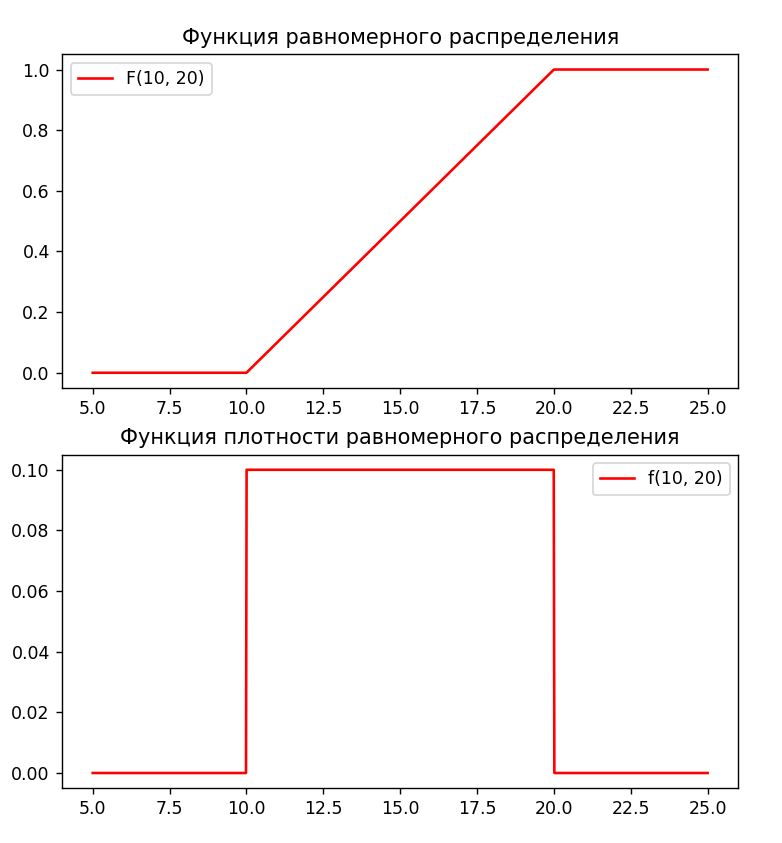
\includegraphics[scale=0.5]{1}
        		\caption{График зависимости температуры $T(x, t_m)$ от координаты $x$}
        		\label{fig:res1}
        	\end{center}
\end{figure}

\item График зависимости $T(x_n, t)$ при нескольких фиксированных значениях координаты $x_n$. 

\begin{figure}[H]
        	\begin{center}
        		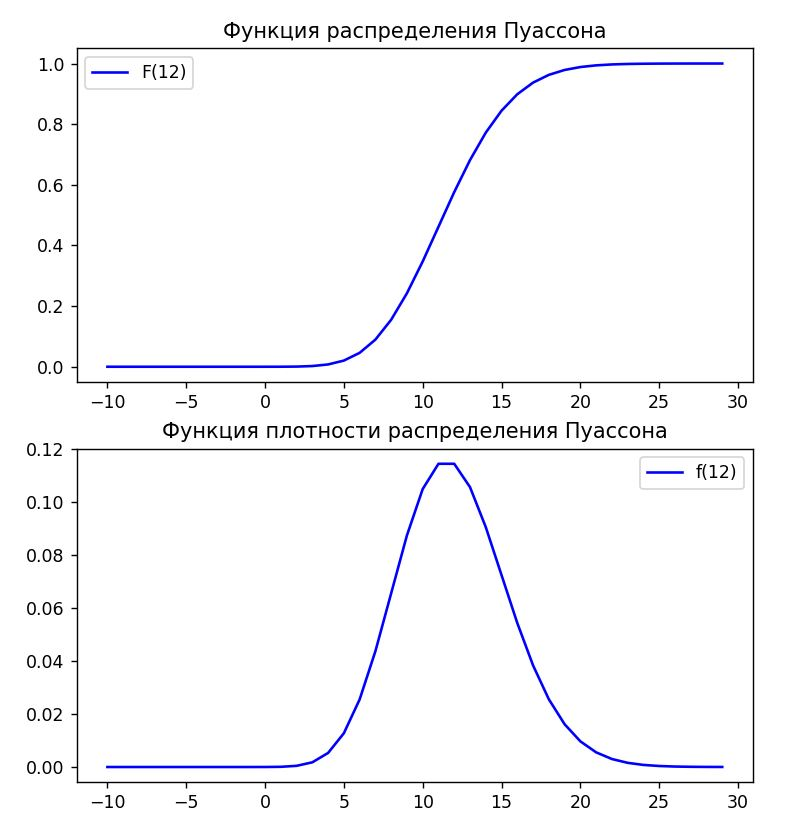
\includegraphics[scale=0.5]{2}
        		\caption{График зависимости  $T(x_n, t)$ при нескольких фиксированных значениях координаты $x_n$}
        		\label{fig:res1}
        	\end{center}
\end{figure}

Верхний график соответствует случаю $x=0$, нижний случаю $x=l$. 

\end{enumerate}


\section*{Ответы на вопросы}

\begin{enumerate}
\item Результаты тестирования программы.\\
Если из полученных разностных аналогов краевых условий обнулить $c(u)$, принять $\tau$ равным 1 и заменить зависимость коэффициента теплопроводности от $T$ на зависимость от координаты на стержне $x$, то можно получить график (Рис. 3), соответствующий полученному графику в 3 лабораторной работе (Рис. 4).
\begin{figure}[H]
        	\begin{center}
        		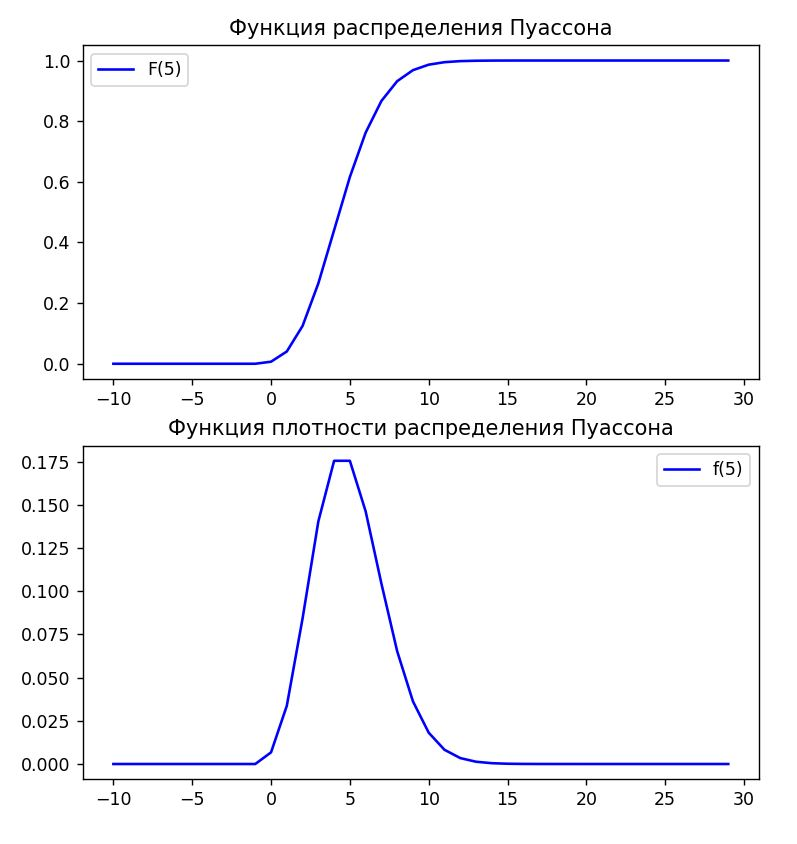
\includegraphics[scale=0.5]{3}
        		\caption{График из 4 лабораторной работы}
        		\label{fig:res1}
        	\end{center}
\end{figure}

\begin{figure}[H]
        	\begin{center}
        		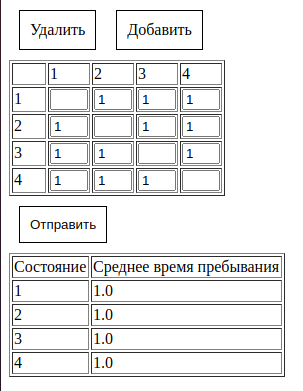
\includegraphics[scale=0.5]{4}
        		\caption{График из 3 лабораторной работы}
        		\label{fig:res1}
        	\end{center}
\end{figure}

\newpage
Если обнулить поток $F_0 (T)$, то на выходе должны получить график температуры, установившейся в соответствии с температурой окружающей среды. (Рис. 5)

\begin{figure}[H]
        	\begin{center}
        		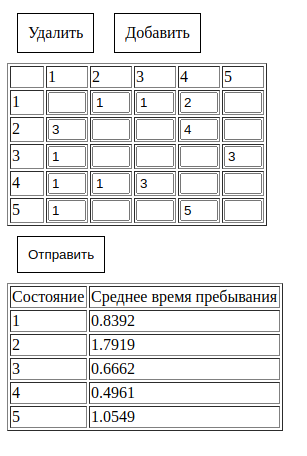
\includegraphics[scale=0.5]{5}
        		\caption{График при нулевом потоке}
        		\label{fig:res1}
        	\end{center}
\end{figure}

\item Выполните линеаризацию уравнения (14.8) по Ньютону, полагая для простоты, что все коэффициенты зависят только от одной переменной $\buildrel\,\,\frown\over{y}_n$.
\end{enumerate}

Уравнение, которое необходимо линеаризовать

\begin{equation}
\begin{cases}
\buildrel\,\,\frown\over{K}_0\buildrel\,\,\frown\over{y}_0+\buildrel\,\,\frown\over{M}_0\buildrel\,\,\frown\over{y}_1=\buildrel\,\,\frown\over{P}_0\\
\buildrel\,\,\frown\over{A}_n\buildrel\,\,\frown\over{y}_{n-1}-\buildrel\,\,\frown\over{B}_n\buildrel\,\,\frown\over{y}_n+\buildrel\,\,\frown\over{D}_n\buildrel\,\,\frown\over{y}_{n+1}=-\buildrel\,\,\frown\over{F}_n, 1\le n\le N-1\\
\buildrel\,\,\frown\over{K}_N\buildrel\,\,\frown\over{y}_N+\buildrel\,\,\frown\over{M}_{N-1}\buildrel\,\,\frown\over{y}_{N-1}=\buildrel\,\,\frown\over{P}_N\\
\end{cases}
\end{equation}

Выполним линеаризацию методом Ньютона по переменным $\buildrel\,\,\frown\over{y}_{n-1}, \buildrel\,\,\frown\over{y}_n, \buildrel\,\,\frown\over{y}_{n+1}$

Обозначим текущую итерацию $s$, а предыдущую итерацию за $(s-1$).  

Начальное распределение задается произвольно $\buildrel\,\,\frown\over{y}_0$. 

Будем полагать, что значения предыдущей итерации известны.\\

Зная, что коэффициенты системы зависят только от $\buildrel\,\,\frown\over{y}_n$, получим

\begin{multline*}
\bigg(\buildrel\,\,\frown\over{A}_n\buildrel\,\,\frown\over{y}_{n-1}-\buildrel\,\,\frown\over{B}_n\buildrel\,\,\frown\over{y}_n+\buildrel\,\,\frown\over{D}_n\buildrel\,\,\frown\over{y}_{n+1}+\buildrel\,\,\frown\over{F}_n\bigg)\bigg|_{(s-1)}+\buildrel\,\,\frown\over{A}_n^{(s-1)}\Delta\buildrel\,\,\frown\over{y}_{n-1}^{(s)}+\\
+\bigg(\frac{\partial \buildrel\,\,\frown\over{A}_n}{\partial\buildrel\,\,\frown\over{y}_n}\buildrel\,\,\frown\over{y}_{n-1}-\frac{\partial \buildrel\,\,\frown\over{B}_n}{\partial\buildrel\,\,\frown\over{y}_n}\buildrel\,\,\frown\over{y}_{n}-\buildrel\,\,\frown\over{B}_n+\frac{\partial \buildrel\,\,\frown\over{D}_n}{\partial\buildrel\,\,\frown\over{y}_n}\buildrel\,\,\frown\over{y}_{n+1}+\frac{\partial \buildrel\,\,\frown\over{F}_n}{\partial\buildrel\,\,\frown\over{y}_n}\bigg)\bigg|_{(s-1)}\cdot
\Delta\buildrel\,\,\frown\over{y}_{n}^{(s)}+ \\
+\buildrel\,\,\frown\over{D}_n^{(s-1)}\Delta\buildrel\,\,\frown\over{y}_{n+1}^{(s)}=0
\end{multline*}

\newpage
Введем обозначения 

\begin{equation*}
\begin{aligned}
&A_n=\buildrel\,\,\frown\over{A}_n^{(s-1)}\\
&B_n=\bigg(-\frac{\partial \buildrel\,\,\frown\over{A}_n}{\partial\buildrel\,\,\frown\over{y}_n}\buildrel\,\,\frown\over{y}_{n-1}+\frac{\partial \buildrel\,\,\frown\over{B}_n}{\partial\buildrel\,\,\frown\over{y}_n}\buildrel\,\,\frown\over{y}_{n}+\buildrel\,\,\frown\over{B}_n-\frac{\partial \buildrel\,\,\frown\over{D}_n}{\partial\buildrel\,\,\frown\over{y}_n}\buildrel\,\,\frown\over{y}_{n+1}+\frac{\partial \buildrel\,\,\frown\over{F}_n}{\partial\buildrel\,\,\frown\over{y}_n}\bigg)\bigg|_{(s-1)}\\
&D_n=\buildrel\,\,\frown\over{D}_n^{(s-1)}\\
&F_n=\bigg(\buildrel\,\,\frown\over{A}_n\buildrel\,\,\frown\over{y}_{n-1}-\buildrel\,\,\frown\over{B}_n\buildrel\,\,\frown\over{y}_n+\buildrel\,\,\frown\over{D}_n\buildrel\,\,\frown\over{y}_{n+1}+\buildrel\,\,\frown\over{F}_n\bigg)\bigg|_{(s-1)}
\end{aligned}
\end{equation*}

Тогда

\begin{equation*}
A_n\Delta\buildrel\,\,\frown\over{y}_{n-1}^{(s)}-B_n\Delta\buildrel\,\,\frown\over{y}_{n}^{(s)}+D_n\Delta\buildrel\,\,\frown\over{y}_{n+1}^{(s)}=-F_n
\end{equation*}

Выполним линеаризацию краевых условий

Для $\buildrel\,\,\frown\over{y}_0$

\begin{multline*}
\bigg( \buildrel\,\,\frown\over{K}_0 \buildrel\,\,\frown\over{y}_0+ \buildrel\,\,\frown\over{M}_0 \buildrel\,\,\frown\over{y}_1- \buildrel\,\,\frown\over{P}_0\bigg)\bigg|_{(s-1)}+\buildrel\,\,\frown\over{K}_0^{(s-1)}\Delta\buildrel\,\,\frown\over{y}_{0}^{(s)}+\buildrel\,\,\frown\over{M}_0^{(s-1)}\Delta\buildrel\,\,\frown\over{y}_{1}^{(s)}=0
\end{multline*}

\begin{equation*}
\begin{aligned}
&K_0=\buildrel\,\,\frown\over{K}_0^{(s-1)}\\
&M_0=\buildrel\,\,\frown\over{M}_0^{(s-1)}\\
&P_0=-\bigg( \buildrel\,\,\frown\over{K}_0 \buildrel\,\,\frown\over{y}_0+ \buildrel\,\,\frown\over{M}_0 \buildrel\,\,\frown\over{y}_1- \buildrel\,\,\frown\over{P}_0\bigg)\bigg|_{(s-1)}\\
\end{aligned}
\end{equation*}

\begin{equation*}
\begin{aligned}
&K_0\Delta\buildrel\,\,\frown\over{y}_{0}^{(s)}+M_0\Delta\buildrel\,\,\frown\over{y}_{1}^{(s)}=P_0\\
\end{aligned}
\end{equation*}

Для $\buildrel\,\,\frown\over{y}_n$

\begin{multline*}
\bigg( \buildrel\,\,\frown\over{K}_N \buildrel\,\,\frown\over{y}_N+ \buildrel\,\,\frown\over{M}_{N-1} \buildrel\,\,\frown\over{y}_{N-1}- \buildrel\,\,\frown\over{P}_N\bigg)\bigg|_{(s-1)}+\buildrel\,\,\frown\over{K}_N^{(s-1)}\Delta\buildrel\,\,\frown\over{y}_{N}^{(s)}+\buildrel\,\,\frown\over{M}_{N-1}^{(s-1)}\Delta\buildrel\,\,\frown\over{y}_{N-1}^{(s)}=0
\end{multline*}

\begin{equation*}
\begin{aligned}
&K_N=\buildrel\,\,\frown\over{K}_N^{(s-1)}\\
&M_{N-1}=\buildrel\,\,\frown\over{M}_{N-1}^{(s-1)}\\
&P_N=-\bigg( \buildrel\,\,\frown\over{K}_N \buildrel\,\,\frown\over{y}_N+ \buildrel\,\,\frown\over{M}_{N-1} \buildrel\,\,\frown\over{y}_{N-1}- \buildrel\,\,\frown\over{P}_N\bigg)\bigg|_{(s-1)}\\
\end{aligned}
\end{equation*}

\begin{equation*}
\begin{aligned}
&K_N\Delta\buildrel\,\,\frown\over{y}_{N}^{(s)}+M_{N-1}\Delta\buildrel\,\,\frown\over{y}_{N-1}^{(s)}=P_N\\
\end{aligned}
\end{equation*}

Получаем систему

\begin{equation}
\begin{cases}
A_n\Delta\buildrel\,\,\frown\over{y}_{n-1}^{(s)}-B_n\Delta\buildrel\,\,\frown\over{y}_{n}^{(s)}+D_n\Delta\buildrel\,\,\frown\over{y}_{n+1}^{(s)}=-F_n\\
K_0\Delta\buildrel\,\,\frown\over{y}_{0}^{(s)}+M_0\Delta\buildrel\,\,\frown\over{y}_{1}^{(s)}=P_0\\
K_N\Delta\buildrel\,\,\frown\over{y}_{N}^{(s)}+M_{N-1}\Delta\buildrel\,\,\frown\over{y}_{N-1}^{(s)}=P_N\\
\end{cases}
\end{equation}

Система решается методом прогонки. Находим все $\Delta \buildrel\,\,\frown\over y_n^s$.
Зная приближение $s-1$, можно найти приближение $s$
$$ \buildrel\,\,\frown\over y_n^s=  \buildrel\,\,\frown\over y_n^{(s-1)}+\Delta \buildrel\,\,\frown\over y_n^s $$

Итерационный процесс завершается, когда достигнуто условие

$\max\bigg|\frac{\Delta \buildrel\,\,\frown\over y_n^s}{\buildrel\,\,\frown\over y_n^s}\bigg|\le\varepsilon$. 

\section*{Вывод}

В ходе лабораторной работы были получены навыки разработки алгоритмов решения смешанной краевой задачи при реализации моделей, построенных на квазилинейном уравнении параболического типа.

\end{document}